\title{Disciplina ``Métodos e Técnicas de Mapeamento Digital de Solos''}
\author{por Waldir de Carvalho Junior, Cesar da Silva Chagas e Michele Duarte de Menezes}
\maketitle
Em função da demanda de uma disciplina sobre o tema junto ao programa de pós-graduação do Departamento de Solos da UFRRJ, fomos solicitados a organizar uma  disciplina abordando o tema de mapeamento digital de solos (MDS) como Tópicos Especiais em Ciência do Solo. Inicialmente, foram realizadas duas reuniões com as Profas. Michele Duarte e Lucia Anjos para definição de uma estratégia para a disciplina e a estrutura para os alunos.\\
Ao todo 15 alunos de pós-graduação se inscreveram, sendo 10 do Departamento de Ciência do Solo e cinco de outros departamentos. Do total de matriculados apenas três alunos não concluíram a disciplina.\\
A disciplina, que na UFRRJ é trimestral (junho a agosto de 2013), teve ao todo 14 aulas com mais duas aulas extras no mês de setembro, perfazendo um total de 56 horas/aula, tempo considerado suficiente para apresentar aos alunos aspectos teóricos e práticos dos principais métodos de predição utilizados no MDS.\\
Inicialmente,  a disciplina apresentou uma breve teoria introdutória sobre mapeamento de solos, tipos e utilizações. Para nivelar os conhecimentos, foram apresentados alguns conceitos básicos de geoprocessamento, úteis para aplicação em mapeamento digital.\\
Uma das premissas do curso foi a utilização de softwares livres e quanto aos equipamentos de hardware, foi solicitado aos alunos que utilizassem seus próprios laptops/ notebooks.\\
A estratégia funcionou a contento já que os alunos puderam acompanhar satisfatoriamente todas as aulas práticas do curso. No entanto, vale ressaltar que  é necessária uma configuração mínima de hardware, de modo que todos os processamentos sejam realizados em tempo hábil durante as aulas.\\
\\
\begin{figure}[htbp]
   \centering
   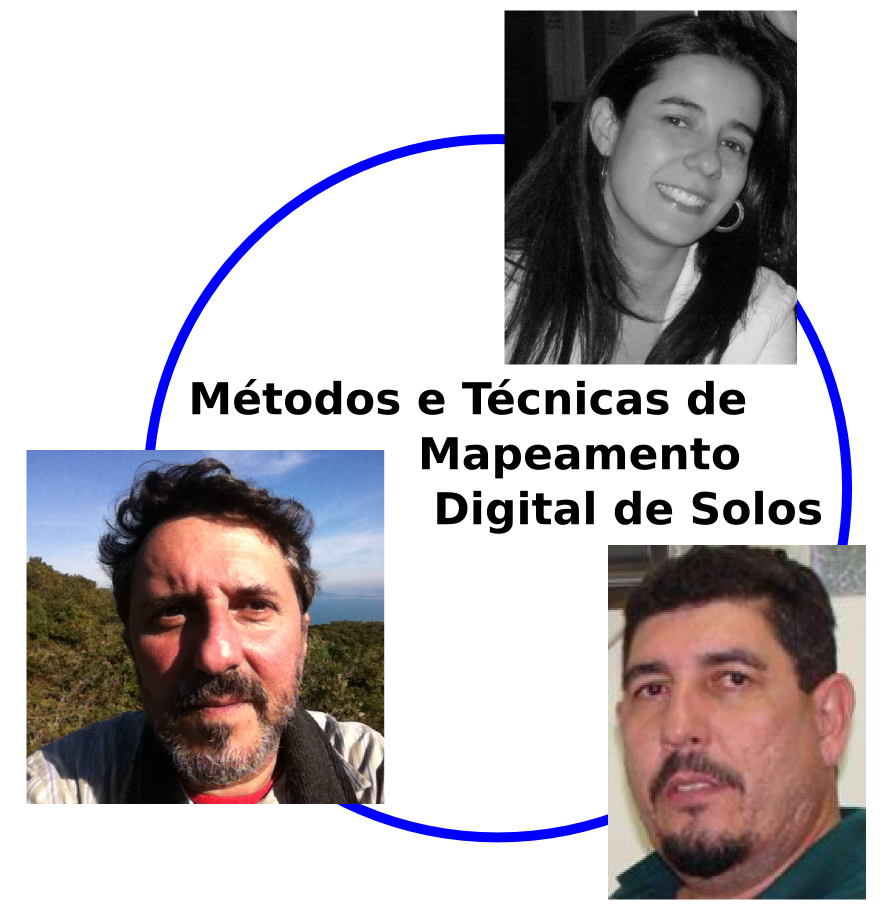
\includegraphics[width=0.95\linewidth]{figuras/trio}
   \caption{O trio de professores.}
   \label{fig:foto-trio}
\end{figure}
\noindent Os seguintes softwares livres foram utilizados: SAGA GIS, R e SoLim. Inicialmente, foram dados aos alunos noções básicas destes softwares, para que eles se habituassem com os mesmos.\\
Nos procedimentos das aulas práticas foi utilizado um conjunto de dados com 101 perfis de solos analisados com resultados de argila e carbono do horizonte A, pertencentes ao projeto Corredor Ecológico do COMPERJ na Bacia do Rio Guapi-Macacu no Estado do Rio de Janeiro.\\
\\
\begin{figure}[htbp]
   \centering
   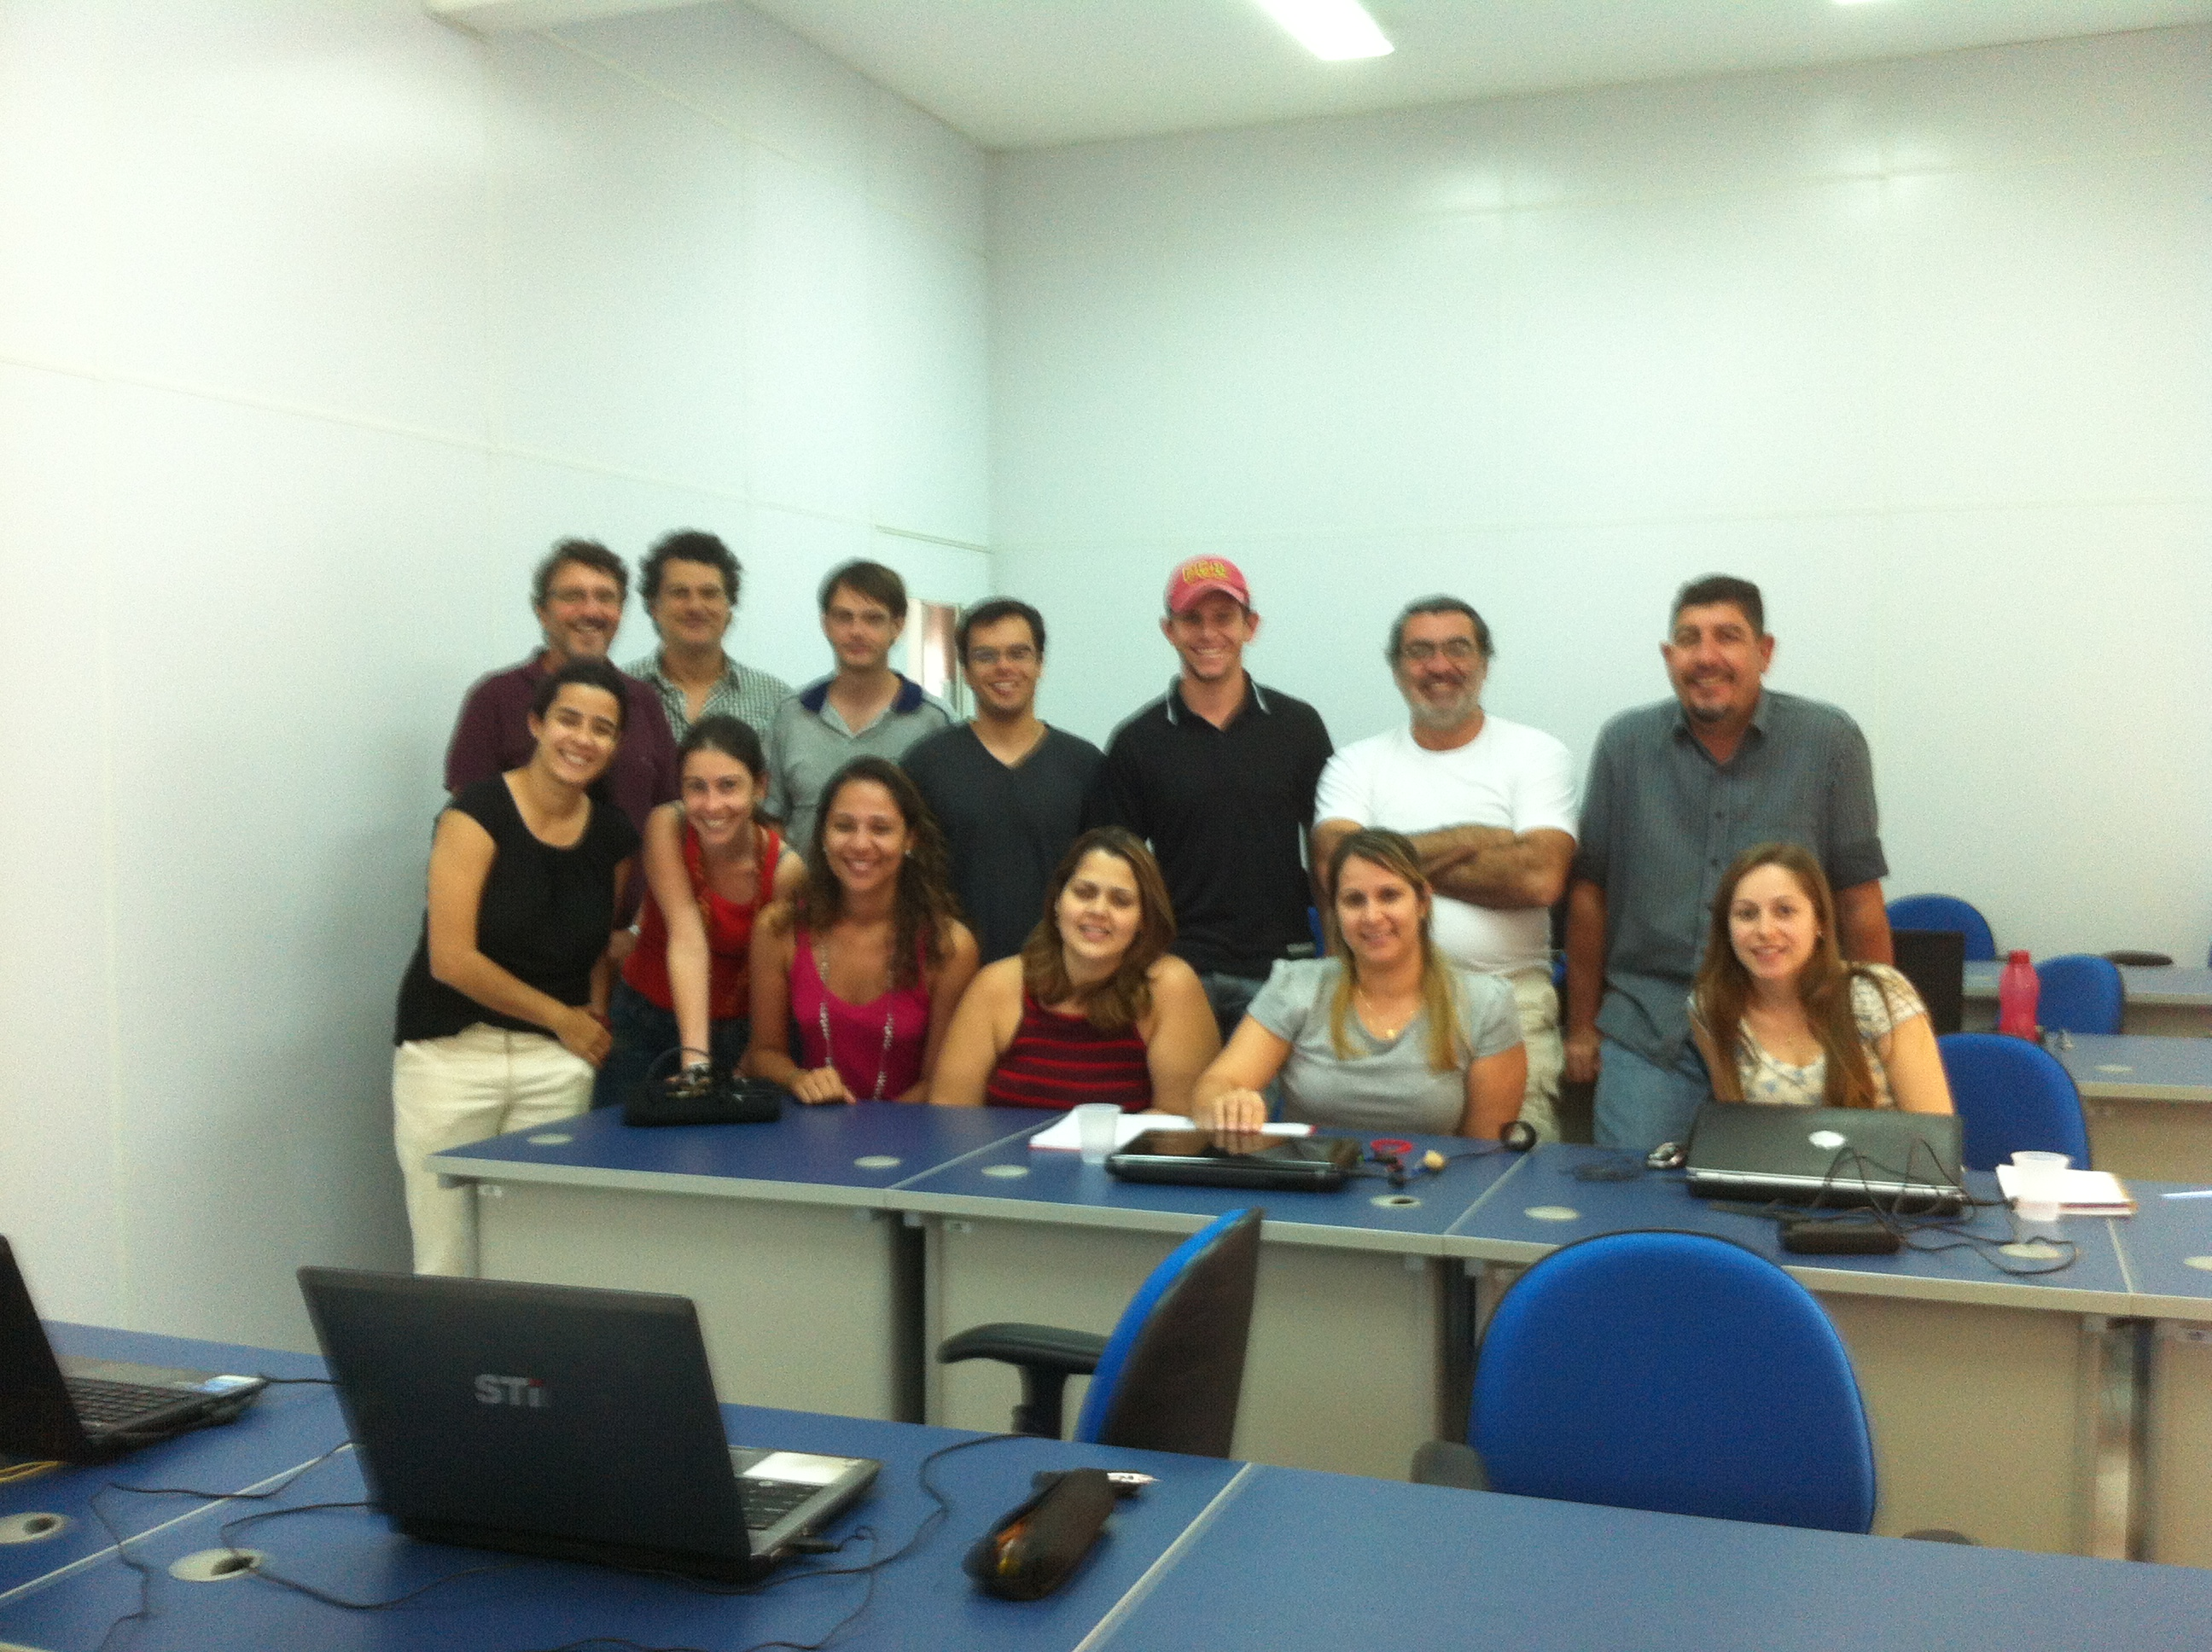
\includegraphics[width=0.95\linewidth]{figuras/foto-waldir.jpg}
   \caption{Foto do grupo.}
   \label{fig:foto}
\end{figure}
\noindent As aulas contemplaram os seguintes temas: Introdução ao Mapeamento Digital de Solos (MDS), Introdução ao uso de ferramentas computacionais livres e abertas para MDS, Variáveis e Covariáveis usadas Mapeamento Digital de Solos, Cálculo de Covariáveis Ambientais usadas em MDS usando ferramentas de SIG, Introdução a Modelagem para MDS, Utilização do SAGA GIS e R na modelagem para MDS, Modelos Lineares Simples e Múltiplos eaplicações do R, Modelos de Árvores de Decisão e Regressão e aplicação no R, Modelos do tipo Random Forest logísticos e de regressão, Random Forest e aplicações no R, Conceitos e Estruturas de Redes Neurais Artificiais, Construção e Aplicação de Redes Neurais Artificiais no pacote RSNNS no R, Introdução aos sistemas SoLIM e Knowledge, Experiências com softwares SoLIM e Knowledge, Mapeamento digital de classes de solos com Redes Neurais, Teoria de Geoestatística e sua interação com mapeamento digital de solos, Aplicação de Geoestatística para mapeamento de atributos do solo, Teoria de cokrigagem 
e regressão-krigagem sua interação com mapeamento digital de solos, Aplicação de de cokrigagem e regressão-krigagem para mapeamento de atributos do solo no R.\\
A disciplina contou também com a participação especial do Dr. Prof. Phillip Owens da Purdue University  que falou sobre sua experiência com mapeamento digital de solos.\\
Como avaliação final da disciplina foi proposto um trabalho prático com dados oferecidos ou próprios dos alunos, em formato de artigo, seguindo as normas da RBCS, a ser entregue até o final de setembro.\\
No final do curso, foi solicitado aos alunos que avaliassem o mesmo, através de um questionário. O resultado da avaliação do curso pelos alunos  mostrou pontos positivos e negativos, detalhados a seguir. A primeira pergunta era: ``Quanto à carga horária, foi satisfatória ou não? A distribuição (04 horas/semana) foi conveniente?''. As respostas em sua maioria (11) foi positiva às duas questões (carga horária e distribuição), entretanto  três alunos sugeriram uma carga horária maior. Apenas um aluno sugeriu que houvesse duas aulas por semana com duas horas cada.\\
A segunda questão foi: ``Em sua avaliação, quais foram as principais dificuldades para acompanhar o curso?'', com as opções de didática, material didático (dados e softwares apresentados durante o curso), carga horária e distribuição, hardware, software, instalações (estrutura), outras (especificar).  A principal dificuldade apontada pelos alunos foi ``software'', seguido por ``hardware'' e ``conhecimentos em mapeamento de solos'' (contida na opção outras). As opções de ``material didático (dados e softwares apresentados durante o curso)'' e ``carga horária e distribuição'' aparecem a seguir. Não foram mencionados a ``didática'' , nem ``instalações (estrutura)''.\\
A terceira questão foi: ``Você acredita que alguma das disciplinas da pós-graduação ou algum conhecimento específico deveriam ser pré-requisitos para o curso? Quais?'' A maioria disse que sim, mas sem que o termo ``pré-requisito'' seja empregado, ficando apenas como sugestão para futuros alunos. Os alunos apontaram as seguintes disciplinas em ordem decrescente de importância: Estatística e Geoestatística Geoprocessamento/SIG, Pedologia, classificação e levantamento de solos, básico de R.\\
A última questão diz: ``A forma de avaliação (trabalho prático apresentado em formato de artigo) está coerente com o curso? Uma apresentação do trabalho para os colegas é interessante?'' A maioria respondeu ``sim'' às duas indagações.\\
A experiência desta primeira disciplina foi  positiva e nos permitiu montar uma estrutura que pode ser aperfeiçoada para uma possível reapresentação da disciplina no próximo ano ou até mesmo em outra instituição que esteja interessada no curso. O esforço de preparação das aulas foi compensado também com nosso aprendizado.\\
A oferta da disciplina de MÉTODOS E TÉCNICAS DE MAPEAMENTO DIGITAL DE SOLOS supriu uma demanda na pós-graduação do Departamento de Ciência do Solo da UFRRJ. Por não se tratar de uma disciplina regular, a procura pode ser considerada satisfatória, com 15 alunos inicialmente matriculados e 12 concluindo o curso.\\
Temos agora um conjunto de dados estruturados, que pode servir de ponto de partida para uma nova oferta desta disciplina.\\

\address{Waldir de Carvalho Junior\\
Embrapa Solos\\
\url{www.cnps.embrapa.br}\\
\email{Waldir.Carvalho@embrapa.br}}\\
\address{Cesar da Silva Chagas\\
Embrapa Solos\\
\email{Cesar.Chagas@embrapa.br}}\\
\address{Michele Duarte de Menezes\\
Universidade Federal Rural do Rio de Janeiro\\
\email{michele\_duarte@ig.com.br}}
%%% Local Variables: 
%%% mode: latex
%%% TeX-master: documento-principal.tex
%%% End: